\chapter*{Chen's Theorem: The Bar Complex by Thomas Wei{\ss}schuh}
%\addcontentsline{toc}{chapter}{**Chen's Theorem: The bar complex by Thomas Wei{\ss}schuh}

Thomas Wei\ss schuh on September 3rd, 2012.

%[Aim of Talk] 

\section{The (unreduced) bar complex}

Let $A^{\bullet}$ be a differential graded algebra, $\Z$-graded with a differential $\partial : A^k \to A^{k+1}$. The degree of an element in $A$ is for short denoted by $|-|$. 
Let also $a, b : A^{\bullet} \to k$ be augmentations. 
Consider the infinite direct sum 
\[
\bigoplus_{r \geq 0} A^{\otimes r} = k \oplus A \oplus A^{\otimes 2} \oplus \ldots
\]
generated by elements written as 
\[ [a_1 \mid \ldots \mid a_r] \in A^{\otimes r}. \]
On this set, one has two graduations: First the usual degree on the tensor product of graded complexes, given by 
\[ \deg_{tensor} : [a_1 \ldots a_r] \mapsto |a_1| + \ldots + |a_r| \] %\sum_{i=1}^r |a_i| \]
and the second, so-called simplicial graduation, given by negative length of the tensor,
\[ \deg_{simpl} : [a_1 \ldots a_r] \mapsto -r. \]

Splitting the above sum up with respect to these to degrees leads to the following array.
\[
\begin{xy}
\xymatrix{
  & {-2} & {-1} & {0} & {\deg_{simpl} / \deg_{tensor}} \\ 
  {\ar[r]} & {\left(A^{\otimes 2} \right)^2 \ar[r]^\delta } & {A^2 \ar[r]^\delta} & {0} & {2} \\
  {\ar[r]} & {\left(A^{\otimes 2} \right)^1 \ar[r]^\delta \ar[u]_\partial} & {A^1 \ar[r]^\delta \ar[u]_\partial} & {0} & {1} \\
  {\ar[r]} & {\left(A^{\otimes 2} \right)^0 \ar[r]^\delta \ar[u]_\partial} & {A^0 \ar[r]^0 \ar[u]_\partial} & {k} & {0} \\
  {\ar[r]} & {\left(A^{\otimes 2} \right)^{-1} \ar[r]^\delta \ar[u]_\partial} & {A^{-1} \ar[r]^\delta \ar[u]_\partial} & {0} & {-1} \\
}\end{xy} 
\]
Here the differentials are given by
\begin{eqnarray*}
\partial : [a_1 \mid \ldots \mid a_r] & \mapsto & \sum_{i=1}^r (-1)^{|a_1| + \ldots + |a_{i-1}| + i} [\ldots \mid \partial a_i \mid \ldots ] \\
\delta : [a_1 \mid \ldots \mid a_r] & \mapsto & \sum_{i=0}^{r} (-1)^{|a_1| + \ldots + |a_i| + i + 1} [\ldots \mid a_i a_{i+1} \mid \ldots]
\end{eqnarray*}
%with the conventian that the sum for $\delta$ in Index reads for the special Indizes $i=0,r$ as
%\[ 
%\]
where in the definition of $\delta$ the terms for $i=0,r$ are defined as follows 
\begin{align*}
i=0 &: \  - a(a_1) [a_2 \mid \ldots \mid a_r] \\
i=r &: \  (-1)^{|a_1|+\ldots +|a_r|+r+1} [a_1 \mid \ldots \mid a_{r-1}] b(a_r) 
\end{align*}
Especially for $r=1,2$, one gets 
\begin{align*}
\delta : 
\begin{aligned} \ 
  [a_1] &\mapsto -a(a_1) + (-1)^{|a_1|} b(a_1) \\
  [a_1 | a_2] &\mapsto -a(a_1)[a_2] + (-1)^{|a_1|} [a_1 \mid a_2] - (-1)^{|a_1| + |a_2|} b(a_2) [a_1] 
  \end{aligned} 
\end{align*}
With these definitions, $\partial^2 = 0$, $\delta^2 = 0$ and $\partial \delta + \delta \partial = 0$, so this defines a double complex. 

Let $B(A, a, b)$ be the associated $\oplus$-Total complex formed by summing diagonals of slope -1 in the above diagram and indexing by the x-intercept.

\section{Hopf algebra structure on the bar complex} 
In what follows the bar complex, up to now defined as a vector space, is equipped with an hopf algebra structure. 

\begin{defn}
The bar complex admits a product
\[
\nabla : [a_1 \mid \ldots \mid a_r] \otimes [a_{r+1} \mid \ldots \mid a_{r+s}] \mapsto \sum_{\mu \in S_{r,s}} (-1)^{\sigma(\mu, a)} [a_{\mu^{-1}(1)} \mid \ldots \mid a_{\mu^{-1}(r+s)}]
\]
where
\begin{align} \label{graded_sign}
   \sigma(\mu,a) = \sum \limits_{\genfrac{}{}{0pt}{2}{i < j}{ \mu(i) > \mu(j) }} (|a_{i}|-1) (|a_{j}|-1)
\end{align}
ist the graded signum of the tupel $a=[a_1 \ldots a_r]$ with respect to the total degree. 
\end{defn}

Remark that the definition of the product doesn't make use of the augmentations. 
To get compatibility with the simplicial differential one assumes that the product is defined on $B(A,a,c) \otimes B(A,c,b)$ and takes values in $B(A,a,b)$. Here $a,b,c$ are arbitrary augmentations of $A$.


This product is 
\begin{itemize}
\item Associative
\item Graded-commtutative
\item Unital with unit given by inclusion $k \to B(A, a, b)$
\item Compatible with the total differential, if $A$ is graded-commutative.
\end{itemize}

\begin{exam} For elements $a,b$ in $A$ one has
\begin{itemize}
\item $\nabla([a] \otimes 1) = [a] = \nabla( 1 \otimes [a] )$
\item $\nabla([a] \otimes [b]) = [a \mid b] + (-1)^{(|a|-1)(|b|-1)}[b \mid a]$
\item If $a$ is of degree $1$, $[a]^n = n! \underset{n}{\underbrace{[a \mid \ldots\mid a]}}$
\end{itemize}
\end{exam} 

\begin{rem}
A $(p,q)$ shuffle $\mu$ can be thought of as a way in a rectangle. 
If one places the $a_1 \ldots a_p$ horizontally and the $a_{p+1}\ldots a_{p+q}$ vertically, then $\mu$ is given by shuffling the two paths together. 
\begin{center}
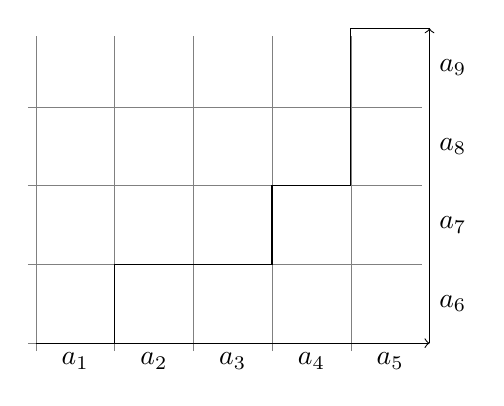
\begin{tikzpicture}[domain=0:5]
    \draw[very thin,color=gray] (-0.1,-0.1) grid (4.9,3.9); %Grid
    \draw[->] (0,0) -- (5,0);     % horizontale Axe
    \draw[->] (5,0) -- (5,4);     % verticale Axe
    \draw (5,0.5) node[right] {$a_6$}
          (5,1.5) node[right] {$a_7$}
          (5,2.5) node[right] {$a_8$}
          (5,3.5) node[right] {$a_9$}; % vertikale Beschriftung
    \draw (0.5,0) node[below] {$a_1$}
          (1.5,0) node[below] {$a_2$}
          (2.5,0) node[below] {$a_3$}
          (3.5,0) node[below] {$a_4$}
          (4.5,0) node[below] {$a_5$}; % horizontale Beschriftung
          
    \draw plot coordinates{(0,0) (1,0) (1,1) (3,1) (3,2) (4,2) (4,4) (5,4)}; %Weg    
\end{tikzpicture}
\end{center}
The signum of the shuffle can be found as the area below this graph. To be more precise, it is $-1$ power the area, which is calculated by giving the segment of $a_i$ the length $|a_i|-1$. 
\end{rem}


\begin{defn}
There is also a coproduct on $B(A, a, b)$:
\begin{align*}
  \Delta : B(A,a,b) &\to B(A,a,c) \otimes B(A,c,b) \\
  [a_1 \mid \ldots \mid a_r] &\mapsto \sum_{i=0}^r [a_1 \mid \ldots \mid a_i] \otimes [a_{i+1} \mid \ldots \mid a_r].
\end{align*}
In the case $i=0$, this should be read as $1 \otimes [a_1 \mid \ldots \mid a_r]$ and similar for $i=r$. 
%In general, one identifies $[] = 1$.
\end{defn}

\begin{exam} \ 
\begin{itemize}
\item $\Delta(1)      = 1 \otimes 1 $
\item $\Delta([a_1])  = 1 \otimes [a_1] + [a_1] \otimes 1 $
\end{itemize}
\end{exam}


It is
\begin{itemize}
\item Co-associative $(\Delta \otimes id) \Delta = (id \otimes \Delta) \Delta$.
\item Compatible with $\epsilon $ = Projection to $k$. $\epsilon$ is the co-unit of the coalgebra. 
\item $\Delta$ is a morphism of complexes ie. it satisfies the co-Leibniz rule.
\end{itemize}

\begin{rem}
The last statement is the reason that the two inner augmentations in the definition of the coproduct have to be equal.
\end{rem}

The algebra and coalgebra structure are compatible with each other, which can be expressed by saying that the coproduct and counit are homomorphisms of unitary algebras. 
In other words, one has a bialgebra-structe on the bar complex. 

\begin{defn} Define the antipode of the bar complex by 
\begin{align*}
S : B(A,a,b) &\to B(A,a,b) \\
[a_1|\ldots |a_r] &\mapsto (-1)^{r+\sigma(s,a)} [a_r | \ldots a_1] 
\end{align*}
where $\sigma(s,a)$ is the graded sign of the permutation $[a_1 \ldots a_r] \mapsto [a_r \ldots a_1]$, see \ref{graded_sign}.
\end{defn}

This antipode gives the bar complex the structure of a hopf algebra.
This means that the following diagram (with $B = B(A,a,b)$ for short) commutes.
\begin{align*}\begin{aligned}%aligned, um nummerierung zu zentrieren 
\begin{xy} \xymatrix{ 
 & B \otimes B \ar[rr]^{S \otimes id} & & B \otimes B \ar[dr]^\nabla \\
B \ar[ur]^\Delta \ar[dr]_\Delta \ar[rr]^\epsilon & & k \ar[rr]^u & & B \\
& B \otimes B \ar[rr]^{id \otimes S}  & & B \otimes B \ar[ur]_\nabla  
} \end{xy} \end{aligned} \end{align*}



\section{The reduced bar complex}

For this section, we assume that $A$ vanishes in negative degree.

Let $D(A, a, b)$ be the subcomplex generated by $[a_1 | \ldots | a_r]$ with at least one $a_i \in A^0$ of degree $0$. As a vectorspace, it is generated by elements $[a_1 | \ldots | a_r]$, some $a_i \in A^0$, and their total differentials.

\begin{defn}[Reduced bar complex]
\[
\overline{B}(A, a, b) = \frac{B(A, a, b)}{D(A, a, b)}
\]
\end{defn}

The subcomplex $D(A, a, b)$ forms an ideal (resp. coideal) for $\nabla$ (resp. for $\Delta$) in $B(A, a, b)$, and consequently gives rise to well defined morphisms of the reduced bar complex. 

To see this, one first observe that the respective property hold for homogenous elements $x \in D(A,a,b)$ with at least one component in degree $0$.
Then use the compatibility of $\nabla$ resp. $\Delta$ with the total differential to see the properties for $\nabla(dx \otimes y)$ and $\Delta(dx)$ respectively (use the first case).



\subsection{An explicit definition of the reduced bar complex.}
On the reduced bar complex, we have two relations. The first relation is 
\[ [ \ldots a_{i-1} | h | a_{i+1} \ldots ] = 0 , \quad  h \in A^0 \] 
Letting $A^+ = A/A^0$ be the positive-degree-part of $A$, this enables one to write
\[ 
      \overline B(A,a,b) = B(A^+, a,b) \mod \text{ additional relations }
\]
with relations arising as differentials of the above elements. 
To be precise, one has the relations
\[
   0 = d[\ldots |h|\ldots ] 
\]
for each $h \in A^0$ (and every possible substitute for $\ldots$).
Explicit description of the total differential gives - modulo the first relation(s) - the additional relations 
\[
     [\ldots a_{i-1} | \partial h | a_{i+1}  \ldots ]
     = [\ldots|a_{i-1}|h a_{i+1}|\ldots] 
     - [\ldots|a_{i-1}h|a_{i+1}|\ldots]
\]
These are all relations that occur.

The schematic picture of the reduced bar complex one should have in mind is


\[
\begin{xy}
\xymatrix{
  {-4} & {-3} & {-2} & {-1} & {0} & {\deg_{simpl} / \deg_{tensor}} \\ 
  \left( A^1 \right)^{\otimes 4} \ar[r]^\delta & \left((A^+)^{\otimes 3} \right)^4 \ar[r]^\delta & \left( (A^+)^{\otimes 2} \right)^4 \ar[r]^\delta &  A^4  \ar[r] &  0  & 4 \\ 
   &   \left(A^1 \right)^{\otimes 3} \ar[r]^\delta \ar[u]_{\partial} & \left((A^+)^{\otimes 2} \right)^3 \ar[r]^\delta \ar[u]_\partial & A^3 \ar[r] \ar[u]_\partial & 0 & 3 \\
   &   & {\left(A^1 \right)^{\otimes 2} \ar[r]^\delta \ar[u]_\partial } & {A^2 \ar[r]} \ar[u]_\partial & {0} & {2} \\
   &   &   & {A^1 \ar[r] \ar[u]_\partial} & {0} & {1} \\
   &   &   &   & k \ar[u]_0  & {0} 
}\end{xy} 
\]

From this, the $0$th cohomology of the reduced bar complex is easy to describe. 
Consider a 0-cocycle $x$ with $x_i$ it's part in simplicial degree $i$. Then one has $\delta x_i = -\partial x_{i+1}$.
Now every summand in $\delta x_i$ and $\partial x_{i+1}$ is an tensor with exactly $1$ degree-$2$ component and degree-$1$-components otherwise. 
Comparing the components shows that the tensor-differential decomposes, i.e. one has $\partial a = a' a''$ for each component $a$ which shows up as a component in a summand of $x$. 
Hence every class in $H^0 \overline{B}(A, a, b)$ is represented by a sum of $[a_1 \mid \ldots \mid a_r]$ with all $|a_i| = 1$ and 
\[
     \partial a_i \in A^1 \cdot A^1  \ \text{ or } \ \partial a_i = 0.
\]
For an element $x = [a_1 \ldots a_r] $ concentrated in a single simplicial degree, one has explicit necessary and sufficient conditions to represent a cohomology class in $H^0 \overline B(A,a,b)$, namely 
\[ 
  x \text{ is cocycle } \iff \text{ all } a_i \text{ closed, and } a_i a_{i+1} = 0 \quad \forall i 
\]


\begin{exam}
Let $V$ be a vector space and $A^\bullet = k \oplus V[-1]$ be the complex $(k \stackrel{0}{\to} V)$, with $k$ set in degree $0$. 
The trivial product gives $A^\bullet$ an DGA structure with augmentation the projection onto $k$. 
Then one has $A^+ = V[-1]$ and the reduced Barkomplex by definition the associated total complex of
\[ \ldots V[-1]^{\otimes 3} \to V[-1]^{\otimes 2} \to  V[-1] \to  k \to 0\]
This as a set equals the set of tensors $T(V)$. 
The total degree of every element $[v_1 | \ldots | v_r]$ equals $0$, so the Barcomplex and $T(V)$ are the same as graded vectorspaces. 
The (total) differential vanishes and one has the hopf algebra structure given by product 
\[ \nabla ([v_1 \ldots v_r] \otimes [v_{r+1} \ldots v_{r+1}]) = \sum_{\mu \in S_{r,s}} [v_{\mu^{-1}} \ldots v_{\mu^{-1}(r+s)}]
\]
since $\sigma(\mu,a) = \sum (1-1)(1-1) = 0$. The antipode is 
\[ S[v_1 \ldots v_r] = (-1)^r [v_r \ldots v_1] 
\] 
and the coproduct formula doesn't specialize. 
\end{exam}

\section{Comparison reduced/unreduced bar complex}

We now compare the two definitions of the bar complex. 
For this we assume $A^{\bullet}$ to be cohomologically connected i.e. graded in non-negative degree's and $H^0(A) = k$. 
The plan is to split the quotient map from the bar-complex to the reduced bar-complex as a composition of two quasi-isomorphism 
\[
B(A, a, b) \to \widetilde{B}(A, a, b) \to \overline{B}(A, a, b).
\]

\begin{itemize}
\item[Step 1.] The maps $s_i : [a_1 \mid \ldots \mid a_r] \mapsto [ a_1 \ldots a_{i-1} \mid 1 \mid a_i \ldots a_r]$ which insert a $1$ in position $i$, together with the simplicial differential, endow the bar-doublecomplex with the structure of a simplicial abelian group. Using the sign-trick and modifying the tensor differential, one even gets the structure of a simplicial complex, i.e. the structure maps are compatible with the tensor differential. 
\[
\xymatrix{
B(A, a, b)^2 \ar@<1cm>[d] \ar@<0cm>[d] \ar@<-1cm>[d] \\
B(A, a, b)^1 \ar@<0.5cm>[u] \ar@<-0.5cm>[u] \ar@<0.5cm>[d] \ar@<-0.5cm>[d] \\
B(A, a, b)^0 \ar[u]
}
\]
By theory of normalization, the image $\widetilde{D}(A, a, b)$ of all degeneration maps $s_i$ (with varying $r$) is acyclic. Now define $\widetilde B(A,a,b)$ as the total complex of the normalization with respect to this simplicial structure, i.e. the total complex of the quotient of the bar-doublecomplex by $\widetilde D(A,a,b)$. 
%Then $\widetilde{B}(A, a, b) = \frac{B(A, a, b)}{\widetilde{D}(A, a, b)}$ is quasi-isomorphic to $B(A, a, b)$.
Sind $\widetilde D$ is acyclic, $\widetilde B(A,a,b)$ is quasi-isomorphic to the unreduced bar complex. 

\item[Step 2.] Now consider the projection $\widetilde B \to \overline B$. 
Filter both complexes by columns. The associated spectral sequence converges to the cohomology of the respective complexes (since they are defined as $\oplus$-totalcomplexes). So it suffices to show, that the above projection is a quasi-isomorphism columnwise. By kunneth, it is enought to look at the tensor-degree-1 case (kunneth is compatible with relations). So one needs $A / k \to A / (A^0 \to dA^0)$ to be an quasi-isomorphism. But its kernel is the complex $(A^0/k \to dA^0)$, which is acyclic since $A$ is asumed to be cohomologically connected. 
%By definition of the maps $s_i$, the complex from step 1 can be written as $\widetilde B(A,a,b) = B(A/k,a,b)$ without further relations. 
%\[
%B(A/k, a, b) \to B(A/(A^0 \to dA^0), a, b)
%\]
%Then $\ker\left(A/k \to \frac{A}{A^0 \to dA^0} \right) = (A^0 \to dA^0)$.
\end{itemize}

\section{The bar complex and iterated integrals}

Let $M$ be a smooth connected manifold and $A^{\bullet}_M$ the differential graded algebra of complex valued differential forms on $M$. 
Assume that two points $a, b \in M$ are given. 
They induce augmentations $a,b : A_M^\bullet \to k$ by setting  
\[
a : 
\begin{array}{rcl} 
\omega & \mapsto & 0 \\
f  & \mapsto & f(a) 
\end{array}
\]

\begin{defn}[Iter]\label{def:iter}
The properties of iterated integrals discussed in talk 2 show that the map 
\[
\iter : 
\begin{array}{rcl}
\Q[\pi_1(M, a, b)] & \to & H^0 \overline{B}(A, a, b)^{\vee} = H^0 B(A, a, b)^\vee \\
\gamma & \mapsto & \left( [a_1 \mid \ldots \mid a_r] \mapsto \int_{\gamma} a_1 \ldots a_r \right)
\end{array}
\]
is well defined. 
\end{defn}
It is not just a map of vector spaces but a map of Hopf algebras, i.e., it respects the product, co-product and antipode. Its dual is given by
\[
\iter^{\vee} : \begin{array}{rcl}
H^0 \overline{B}(A, a, b) & \to & \C \otimes \cO( \pi_1(M, a, b)^{un}) \\
\textrm{$[a_1 \mid \ldots \mid a_r]$} & \mapsto & \left( \gamma \mapsto \int_{\gamma} a_1 \ldots a_r \right)
\end{array}
\]
An equivalent version of Chen's theorem is 
\begin{thm}[Chen]
The morphism $\iter^{\vee}$ is an isomorphism.
\end{thm}



\section{The bar complex and relative cohomology}
Let $n$ be a natural number, and let
\[
Y_i = \left\{ \begin{array}{ll}
\{ (x_1, \ldots, x_n) \in M^n \mid x_i = x_{i+1} \}, & i = 1, \ldots, n-1 \\
\{ (a, x_2, \ldots, x_n) \in M^n \}, & i =0 \\
\{ (x_1, \ldots, x_{n-1}, b) \in M^n \}, & i = n
\end{array} \right.
\]
Then
\[
H^0 B(A, a, b) \to \C \otimes_{a, b} \lim_n H^n(M^n, Z_{ab})
\]
where $Z_{ab} = \cup_{i=0}^n Y_i$. 
We calculate the singular cohomology of $M^n$ relative to $Z_{ab}$, which is by definition the cohomology of the kernel of the restriction of singular cochains to $Z_{ab}$,
%\[
%\begin{array}{rcl}
%H^*(M^n, Z_{ab}) & = & H^* \ker(S^* M^n \to S^* Z_{ab}) \\
%& = & H^* \textrm{Tot}(S^* M^n \to \oplus_i S^*(Y_i) \to \oplus_{i < j} S^*(Y_i \cap Y_j) \to \cdots S^*(Y_0 \cap \cdots \cap Y_n)) \\
%& = & H^* \textrm{Tot}(A_M^{\otimes n} \to \oplus A_M^{\otimes n-1} \to \oplus_{i < j} A_M^{\otimes n-2} \to \cdots
%\end{array}
%\]
\begin{align*}
H^*(M^n, Z_{ab}) & = H^* \ker(S^* M^n \to S^* Z_{ab}) \\
& = H^* \textrm{Tot}(S^* M^n \to \oplus_i S^*(Y_i) \to \oplus_{i < j} S^*(Y_i \cap Y_j) \to \cdots S^*(Y_0 \cap \cdots \cap Y_n)) 
\end{align*}
The second equality can be seen as follows. 
Restriction gives a quasi-isomorphism $S^{\bullet}(Z_{ab}) \to S^{\bullet}(Y_0 + \ldots + Y_n)$ which goes into the group of singular cochains defined over singular chain whose image lies completely in one of the $Y_i$. This essentially follows from the barycentric subdivision of chains. 
Now the Mayer-Vietoris exact sequence allows to replace $S^\bullet(Y_0 + \ldots + Y_n)$ by the above complex, with differentials given by alternating restrictions.  

By integrating one gets a quasi-Isomorphism between complexes
\[
\begin{xy}
\xymatrix{
S^* M^n \ar[r] & \oplus_i S^*(Y_i) \ar[r] & \oplus_{i < j} S^*(Y_i \cap Y_j) & \cdots & S^*(Y_0 \cap \cdots \cap Y_n) \\
A_{M^{n}} \ar[r] \ar[u] & \oplus A_{Y_i} \ar[r] \ar[u] & \oplus_{i < j} A_{Y_i \cap Y_j} \ar[u] & \cdots & A_{Y_0 \cap \ldots \cap Y_n} \ar[u]
}
\end{xy}
\]
inducing an quasi-isomorphism on total complexes. Observe that $Y_{i_1} \cap \ldots \cap Y_{i_r} \cong M^{n-r}$. 
So by the K\"unneth formula, one finally has an isomorphism 
\begin{align*}
H^* \textrm{Tot}(A_M^{\otimes n} \to \oplus A_M^{\otimes n-1} \to \oplus_{i < j} A_M^{\otimes n-2} \to \cdots) \xrightarrow{\cong} H^* (M^n, Z_{ab})
\end{align*}
which is essentially just the integration map. 

There is a short exact sequence of complexes,
\[
\xymatrix{
0 \ar[d] & & & \\
\widetilde{K}_n^{-} \ar[d] & A_M^{\otimes n} \ar@{=}[d] \ar[r] & \cdots \ar[r] & \text{kernel} \ar[d]  \\
\widetilde{K}_n \ar[d] & A_M^{\otimes n} \ar[r] & \cdots \ar[r] & \oplus_{n+1} \C \ar[d] \\
\C_{a,b}[-n] \ar[d]  & 0 \ar[r] & \cdots \ar[r] & \C_{a, b} \\
0 & & &
}
\]
where $kernel$ denotes the kernel of the rightmost map in [---], which in the above diagram is the map to $\C_{a,b}$. 
Note that $kernel$ sits in degree $n$ and so by definition $\widetilde{K}_n^{-}$ calculates $H^n(M^n, Z_{ab})$. Furthermore the cohomology of $\widetilde K_n$ and $\widetilde K_n^-$ agree in degree $>n$. Taking the long exact sequence associated to the short exact sequence gives,
\[
H^{n-1}(\C[-n]) \to H^n(\widetilde{K}_n^-) \to H^n(\widetilde{K}_n) \to H^n(\C_{a, b}[-n])  \stackrel{0}{\to} \cdots
\]
The rightmost map is zero, because the following morphism is an identity. Hence
\[
\C_{a, b} \oplus H^n(M^n, Z_{ab}) = H^n(\widetilde{K}_n) 
\]
%\[
%\begin{array}{rcl}
%\C_{a, b} \oplus H^n(M^n, Z_{ab}) = H^n(\widetilde{K}_n) & \to & H^n F^{-n} B(A, a, b) \\
%(a_1, \ldots, a_r) & \mapsto & a_1 + \cdots + a_r
%\end{array}
%\]
%This map is used to compare two versions of Chen's theorem.
Fact: "Doing the summation" gives an quasi-isomorphism of complexes $\widetilde{K}_n \to F^{-n} \widetilde B (A,a,b)$. Here $F^{-n} \widetilde{B}(A,a,b)$ denotes the truncated subcomplex of elements simplicial degree $\geq -n$.
Taking inductive limit (which is compatible with taking cohomology) gives
\[
    H^0 B(A_M,a,b) = \varinjlim_n F^{-n} \widetilde B(A_M,a,b) = \varinjlim_n \C_{a,b} \oplus H^n (M^n,Z_{ab})
\] 


\begin{rem} It seems that the isomorphism constructed above makes the following diagram commute. 
So Chen's theorem is equivalent for $\iter^\vee$ to be an isomorphism.
\[
\begin{xy}
\xymatrix{
H^0\overline B(A_M,a,b) \ar[rd]^{\iter^\vee} \ar[rr] & & \C_{a,b} \oplus H^n(M^n, Z_{ab}) \ar[ld]_{c^\vee} \\
& \C \otimes \cO [\pi_1(M,a,b)]^\vee 
}
\end{xy}
\]
\end{rem}
